\section{Parameter Passing}

\begin{definition}{Parameter Passing Methods}\\
Data can be passed between functions through:
\begin{itemize}
  \item \textbf{Registers}: Fast, limited number available \\ $\rightarrow$ Caller and Callee use the same register
  \item \textbf{Global Variables}: Shared memory space
  \item \textbf{Stack}: 
    \begin{itemize}
      \item Caller: PUSH parameters onto stack
      \item Callee: Access parameter via LDR from stack
    \end{itemize}
\end{itemize}
\end{definition}

\begin{concept}{Global variable approach}

\begin{minipage}{0.5\linewidth}
NOT recommended!!
\vspace{2mm}\\
\begin{itemize}
  \item Shared variables in dara area
  \item Overhead to access variable
  \item Error prone, unmaintainable
\end{itemize}
\end{minipage}
\begin{minipage}{0.5\linewidth}
  \vspace{-4mm}
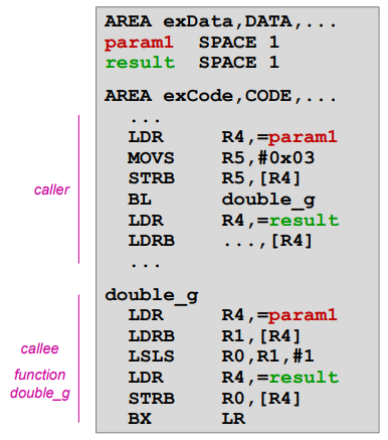
\includegraphics[width=0.8\linewidth]{images/global_variables.png}
\end{minipage}
\end{concept}

\begin{concept}{Register-based approach} (preferred):
  There are two main approaches in Register-based approach:
  by value or by reference
\begin{lstlisting}[language=armasm, style=basesmol]
func    PUSH    {R4, LR}    ; Save registers
        ; R0 contains input parameter
        MOV     R4, R0      ; Save parameter
        ; Process value in R4
        MOV     R0, R4      ; Set return value
        POP     {R4, PC}    ; Restore and return
\end{lstlisting}
\end{concept}

\begin{KR}{Parameter Passing by Value vs. Reference}

\begin{minipage}{0.5\linewidth}
\begin{itemize}
  \item \textbf{Pass by Value}:
    \begin{itemize}
      \item Copies value to function
      \item Changes don't affect original
      \item Default in C
      \item Example: \\Simple types, integers
      \item Limited numbers of registers
    \end{itemize}
  \item \textbf{Pass by Reference}:
    \begin{itemize}
      \item Passes memory address
      \item Changes affect original value
      \item In C: Using pointers
      \item Example: \\Arrays, large structures
    \end{itemize}
\end{itemize}
\end{minipage}
\begin{minipage}{0.5\linewidth}
  \center
pass by value:

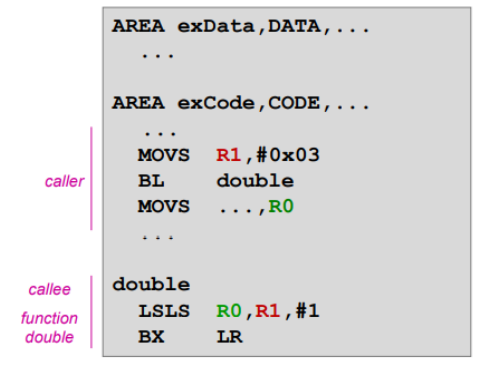
\includegraphics[width=\linewidth]{images/register_passbyval.png}
\end{minipage}

Example implementation:
\begin{lstlisting}[language=armasm, style=basesmol]
; Pass by value
func1   PUSH    {LR}
        ADDS    R0, #1      ; Modify parameter
        POP     {PC}        ; Original unchanged
; Pass by reference
func2   PUSH    {LR}
        LDR     R1, [R0]    ; Load from address
        ADDS    R1, #1      ; Modify value
        STR     R1, [R0]    ; Store back to address
        POP     {PC}        ; Original changed
\end{lstlisting}
\end{KR}


\begin{definition}{ARM Procedure Call Standard}\\
\textbf{Parameter Passing:}
\begin{itemize}
  \item Caller copies parameters from R0 to R3
  \item Caller copies additional parameters to stack
\end{itemize}

\textbf{Return Values:}
\begin{itemize}
  \item \textbf{Small Values} ($\leq$ 32 bits $\rightarrow$ smaller than word size): 
    \begin{itemize}
      \item Return in R0
      \item Zero/sign extend to word if needed
    \end{itemize}
  \item \textbf{Word} (32 bits): return in R0
  \item \textbf{Double Word} (64 bits): return in R0/R1
  \item \textbf{128-bit Values}: return in R0-R3
  \item \textbf{Composite data types} (structs, arrays): 
    \begin{itemize}
      \item Up to 4 bytes: return in R0
      \item Larger: return pointer in R0 (stored in data area)
    \end{itemize}
\end{itemize}

\textbf{Register Usage:}
\begin{itemize}
  \item \textbf{R0-R3}: Arguments/results (caller-saved)
  \item \textbf{R4-R11}: Local variables (callee-saved)
  \item \textbf{R12}: IP - scratch register
  \item \textbf{R13}: SP - stack pointer
  \item \textbf{R14}: LR - link register
  \item \textbf{R15}: PC - program counter
\end{itemize}

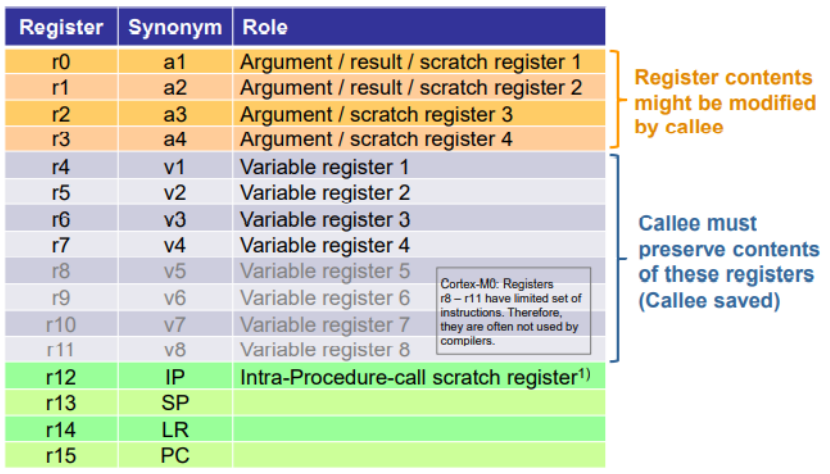
\includegraphics[width=\linewidth]{images/register-usage.png}
\end{definition}

\begin{concept}{Stack Frame Organization}
Complete stack frame layout:

\begin{minipage}[t]{0.5\textwidth}
\textbf{Current Frame:}
    \begin{itemize}
      \item Arguments 5+
      \item Return address (LR)
      \item Saved registers (R4-R11)
      \item Local variables
      \item Temporary storage
    \end{itemize}
\end{minipage}
\begin{minipage}[t]{0.5\textwidth}
\begin{itemize}
  \item \textbf{Previous Stack Frame:}
    \begin{itemize}
      \item Local variables
      \item Saved registers
    \end{itemize}
  \item \textbf{Next Frame:}
    \begin{itemize}
      \item Space for called functions
    \end{itemize}
\end{itemize}
\end{minipage}
\end{concept}

\begin{KR}{Implementing Function Calls}
Steps for calling functions:

\begin{minipage}[t]{0.5\textwidth}
  \textbf{Caller's responsibilities:}
    \begin{itemize}
      \item Place parameters in R0-R3
      \item Push additional parameters \\on stack
      \item Save caller-saved registers \\if needed
    \end{itemize}
\end{minipage}
\begin{minipage}[t]{0.5\textwidth}  
  \textbf{Callee's responsibilities:}
    \begin{itemize}
      \item Save callee-saved registers used
      \item Save LR if making other calls
      \item Process parameters
      \item Place return value in R0
      \item Restore saved registers
    \end{itemize}
\end{minipage}
\end{KR}

\begin{remark}
Important considerations:
\begin{itemize}
  \item Avoid global variables for parameter passing
  \item Use registers for efficiency
  \item Follow ARM calling convention strictly
  \item Consider stack usage in recursive functions
\end{itemize}
\end{remark}

\begin{definition}{Subroutine Call} Caller Side\\
Pattern as used by the compiler. Manually written code may differ.

  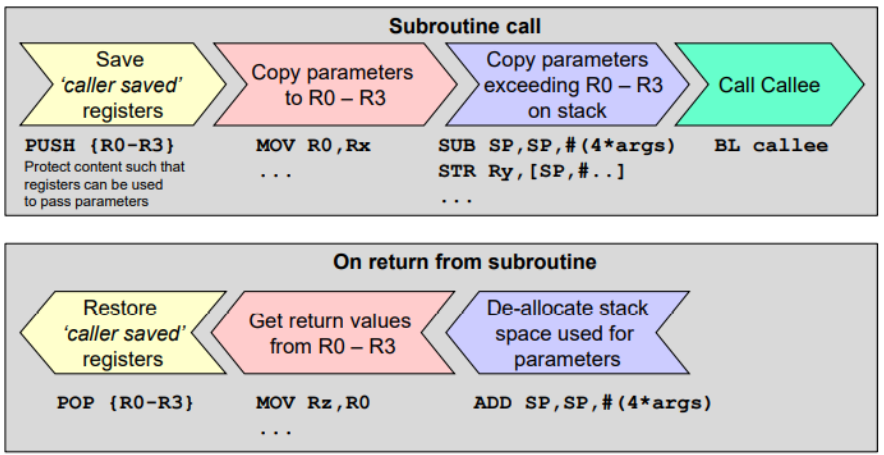
\includegraphics[width=\linewidth]{images/subroutine_call_callerside.png}
\end{definition}


\begin{KR}{Function Parameter Guidelines}
Best practices for parameter passing:

\begin{minipage}[t]{0.45\textwidth}  
\textbf{1. Register Usage:}
\begin{itemize}
  \item R0-R3: First four parameters
  \item R0: Return value
  \item R4-R11: Preserve if used
\end{itemize}
\end{minipage}
\begin{minipage}[t]{0.54\textwidth}
  \textbf{3. Memory Structures:}
\begin{itemize}
  \item Pass pointers for large structures
  \item Use registers for small values
  \item Consider alignment requirements
\end{itemize}
\end{minipage}

\textbf{2. Stack Usage:}
\begin{itemize}
  \item Additional parameters pushed right to left
  \item Maintain 8-byte alignment
  \item Caller responsible for cleaning up stack
\end{itemize}



Example implementation:
\begin{lstlisting}[language=armasm, style=basesmol]
; void func(int a, int b, int c, int d, int e)
; First four params in R0-R3, fifth on stack
func    PUSH    {R4-R6, LR} ; Save registers
        ; Save parameters
        MOV     R4, R0      ; Save a
        MOV     R5, R1      ; Save b
        MOV     R6, R2      ; Save c
        ; R3 contains d
        LDR     R0, [SP, #16] ; Load e from stack
        
        ; Function body
        POP     {R4-R6, PC} ; Return
\end{lstlisting}
\end{KR}

\begin{concept}{Reentrancy}
Handling recursive function calls:
\begin{itemize}
  \item Each call needs its own data set
  \item Registers/globals get overwritten
  \item Solution: ARM Procedure Call Standard
\end{itemize}
\end{concept}

\begin{example2}{Recursive Function Implementation}
Factorial calculation:
\begin{lstlisting}[language=armasm, style=basesmol]
; uint32_t factorial(uint32_t n)
; Input in R0, result in R0
factorial
    PUSH    {R4, LR}        ; Save registers
    MOVS    R4, R0          ; Save n
    CMP     R4, #1          ; Check base case
    BLE     fact_end        ; Return 1 if n <= 1
    
    SUBS    R0, R4, #1      ; n-1
    BL      factorial       ; Recursive call
    MULS    R0, R4, R0      ; n * factorial(n-1)
    
fact_end
    POP     {R4, PC}        ; Restore and return
\end{lstlisting}
\end{example2}


\subsubsection{Parameter Passing Examples}

\begin{example2}{Complex Parameter Example}
Function with mixed parameter types:
\begin{lstlisting}[language=C, style=basesmol]
typedef struct {
    int32_t x;
    int32_t y;
} point_t;

int32_t calculate(point_t* p, int32_t scale, 
                  int32_t* result);
\end{lstlisting}

Assembly implementation:
\begin{lstlisting}[language=armasm, style=basesmol]
; R0 = point_t* p
; R1 = scale
; R2 = result pointer
calculate
    PUSH    {R4-R5, LR}     ; Save registers
    
    ; Load structure members
    LDR     R4, [R0, #0]    ; Load p->x
    LDR     R5, [R0, #4]    ; Load p->y
    
    ; Perform calculation
    MULS    R4, R1, R4      ; x * scale
    MULS    R5, R1, R5      ; y * scale
    
    ; Store result
    STR     R4, [R2, #0]    ; *result = x
    ADDS    R0, R4, R5      ; Return sum
    
    POP     {R4-R5, PC}     ; Return
\end{lstlisting}
\end{example2}



\begin{example2}{Data Structure Access}
Working with structures and arrays:
\begin{lstlisting}[language=C, style=basesmol]
typedef struct {
    uint32_t minutes;
    uint32_t seconds;
} time_t;

time_t time;
\end{lstlisting}

Assembly implementation:
\begin{lstlisting}[language=armasm, style=basesmol]
    ; Access structure members
    LDR     R0, =time       ; Get structure address
    LDR     R1, [R0, #0]    ; Load minutes
    LDR     R2, [R0, #4]    ; Load seconds
    
    ; Modify structure
    ADDS    R2, #1          ; Increment seconds
    CMP     R2, #60         ; Check for overflow
    BLT     store_back
    MOVS    R2, #0          ; Reset seconds
    ADDS    R1, #1          ; Increment minutes
store_back
    STR     R1, [R0, #0]    ; Store minutes
    STR     R2, [R0, #4]    ; Store seconds
\end{lstlisting}
\end{example2}





